\documentclass[10pt,a4paper]{article}
\usepackage[utf8]{inputenc}
\usepackage{amsmath}
\usepackage{amsfonts}
\usepackage{amssymb}
\usepackage{graphicx}
\usepackage{subfigure}
\usepackage{amsmath}
\usepackage{mathrsfs}
\DeclareRobustCommand{\orderof}{\ensuremath{\mathcal{O}}}
\bibliographystyle{prsty}
\usepackage[top=1in, bottom=1in, left=1in, right=1in]{geometry}

\begin{document}
\section{Introduction}
\textbf{ban} is a task of application level. It can calculate band structure along a particular k-path. Because \textbf{ban} will output huge data. We will not attach all output in this file but just keep the output variable name. One may check any \textbf{ban} file in the examples for details. 

\section{Dictionary}

\subsection{Input}
\textit{\textbf{ban.Format}} This parameter tells PiLab how do you define the k-path. There are two options: 'coefficient' or 'coordinate'. Any k-point can be represented by $\textbf{k}=c_{1}\textbf{b}_{1}+c_{2}\textbf{b}_{2}+c_{3}\textbf{b}_{3}$. If 'coefficient', you input values in \textbf{ban.Path} will be interpreted as $[c_{1},c_{2},c_{3}]$. If 'coordinate', it will be interpreted as $[k_{x},k_{y},k_{z}]$. By default, this parameter is set 'coefficient'. \\ \\
\textit{\textbf{ban.Path}} This parameter defines the k-path. The k-path is defined by connecting many k-points. So just input all the k-points you want to go through, PiLab will automatically generate k-mesh along these path.\\ \\
\textit{\textbf{ban.Div}} This parameter defines how many k-points between two input k-points.\\ \\
\textit{\textbf{ban.DivType}} This parameter tells PiLab how to divide each k-path. 'unit' or 'all'. If 'unit', it divide each unit length in k-space into ban.Div k-points. If 'all', it divide a whole k-path, e.g $[0,0,0]$ to $[1,1,1]$ into ban.Div k-points. Note that, the length of k-space are defined by the reciprocal lattice times lattice constant. Therefore all axis ranges from 0 to $2\pi$. So the are independent of lattice constant.\\ \\
\textit{\textbf{ban.Draw}} This parameter tells PiLab whether you want to draw band structures. 'on' or 'off'. Default value is 'on'.\\ \\
\textit{\textbf{ban.Shift}} This parameter tells PiLab whether you want to shift Fermi level to zero in the band structure plot. Note that, this is just a shift in the plot. The original data will not be changed. 

\subsection{Output}
\textit{\textbf{ban.k\_path\_div}} This variable tells how many k-points are generated in each k-path.\\ \\
\textit{\textbf{ban.k\_point}} This variable lists all k-points. Each row vector contains 4 elements [label, $k_{x}$, $k_{y}$, $k_{z}$]. The first just shows it is the n-th k-point. \\ \\
\textit{\textbf{ban.k\_band}} This variable shows the band energies. Each column vector is the band energies of a particular k-point. For example, if there are 100 k-point in total and each k-point has 10 energy levels. Then it would be a 10x100 matrix. The n-th column is the band energies of the n-th k-point shown in ban.k\_point. \\ \\
\textit{\textbf{ban.k\_vec(:,:,n)}} This is the eigenvector matrix of the n-th k-point. Also, if there are 10 bands at each k-point, it would be a 10x10 matrix.\\ \\  


\begin{figure}[tbp]
\centering
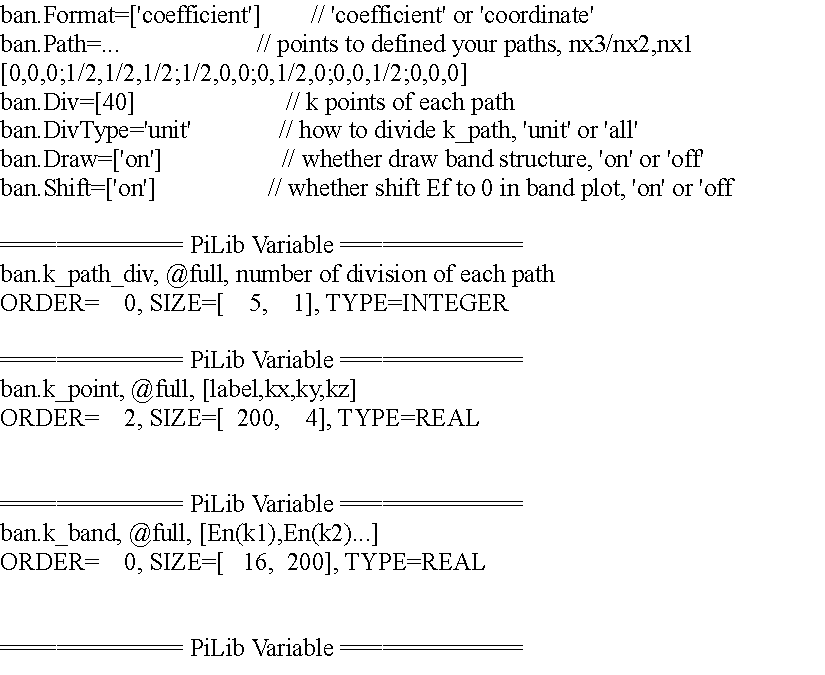
\includegraphics[width=0.9\columnwidth]{NiO_ban.pdf}
\caption{page 1 of NiO\_ban.plb}
\end{figure}

\end{document}